\chapter{Background}
This chapter provides the necessary background on stencil computations and the unique architectural features of the Cerebras Wafer-Scale Engine (\ac{wse}).
\section{Stencil Computations}
Stencil computations are a class of algorithms defined by a regular data access pattern on a grid.
The value of every cell is iteratively updated based on a fixed pattern of its neighbors' values from the previous step.
This pattern is known as the stencil.

These can be categorized by several properties, including the dimensionality of the grid, the shape and locality of the stencil, and the boundary conditions applied.
This thesis focuses on a specific, yet widely applicable, category: \textbf{linear, two-dimensional, star-shaped stencils}.
This means the computation is performed on a 2D grid, where each cell is updated using only its axis-aligned neighbors (i.e., no diagonals), and the new cell value is a linear combination of its previous value and its neighbors' values.
Stencils that also include diagonal neighbors are referred to as box-shaped stencils.

The boundary condition defines how cells at the edges of the grid are handled.
A widely used example is the Dirichlet boundary condition, where edge cells are held to a constant value.
This is the sole boundary condition used in this work.

Stencils are further defined by their radius, which specifies the maximum distance between the center cell and any neighbor used in the update.
We can further categorize the stencils by the parameters.
The stencil's coefficients (or weights) can also be characterized:

\begin{itemize}
    \item If the coefficients for all neighboring cells depend only on their distance from the center, the stencil is symmetric. Otherwise, it is asymmetric. Asymmetric stencils are crucial for modeling direction-dependent phenomena, such as in advection problems.
    \item If the coefficients are the same for all cells across the grid, they are constant. If they depend on the cell's absolute position, they are variable coefficients, used to model problems with spatially varying properties, like heterogeneous materials.
\end{itemize}

A primary application of 2D star-shaped stencils is the finite-difference discretization of the Laplacian operator, which is fundamental to solving \acp{pde} like the Heat Equation and Poisson's Equation. The Heat Equation describes temperature diffusion, with applications in semiconductor chip design, while Poisson's Equation is used in fields like electrostatics and fluid dynamics.

Stencil codes can be broadly classified by their iterative method. In time-stepping applications, each full-grid update (iteration) represents a discrete step forward in time. Such applications are typically run for a fixed number of iterations. The simplest method for this, which updates the entire grid based on the previous state, is the Jacobi method. Its perfectly parallel nature makes it an ideal candidate for massively parallel architectures.

In contrast, relaxation methods iterate until the grid converges to a steady state. Since the notion of discrete time steps is less strict, methods like the Gauss-Seidel or multigrid methods can be employed to accelerate convergence. These methods often introduce dependencies that break the perfect parallelism of the Jacobi method. While the \ac{wse} could be adapted for such methods, they typically require a global convergence check (an all-reduce operation), which is beyond the scope of this thesis. Therefore, this work focuses exclusively on Jacobi-style updates.

\begin{figure}[h]
    \centering
    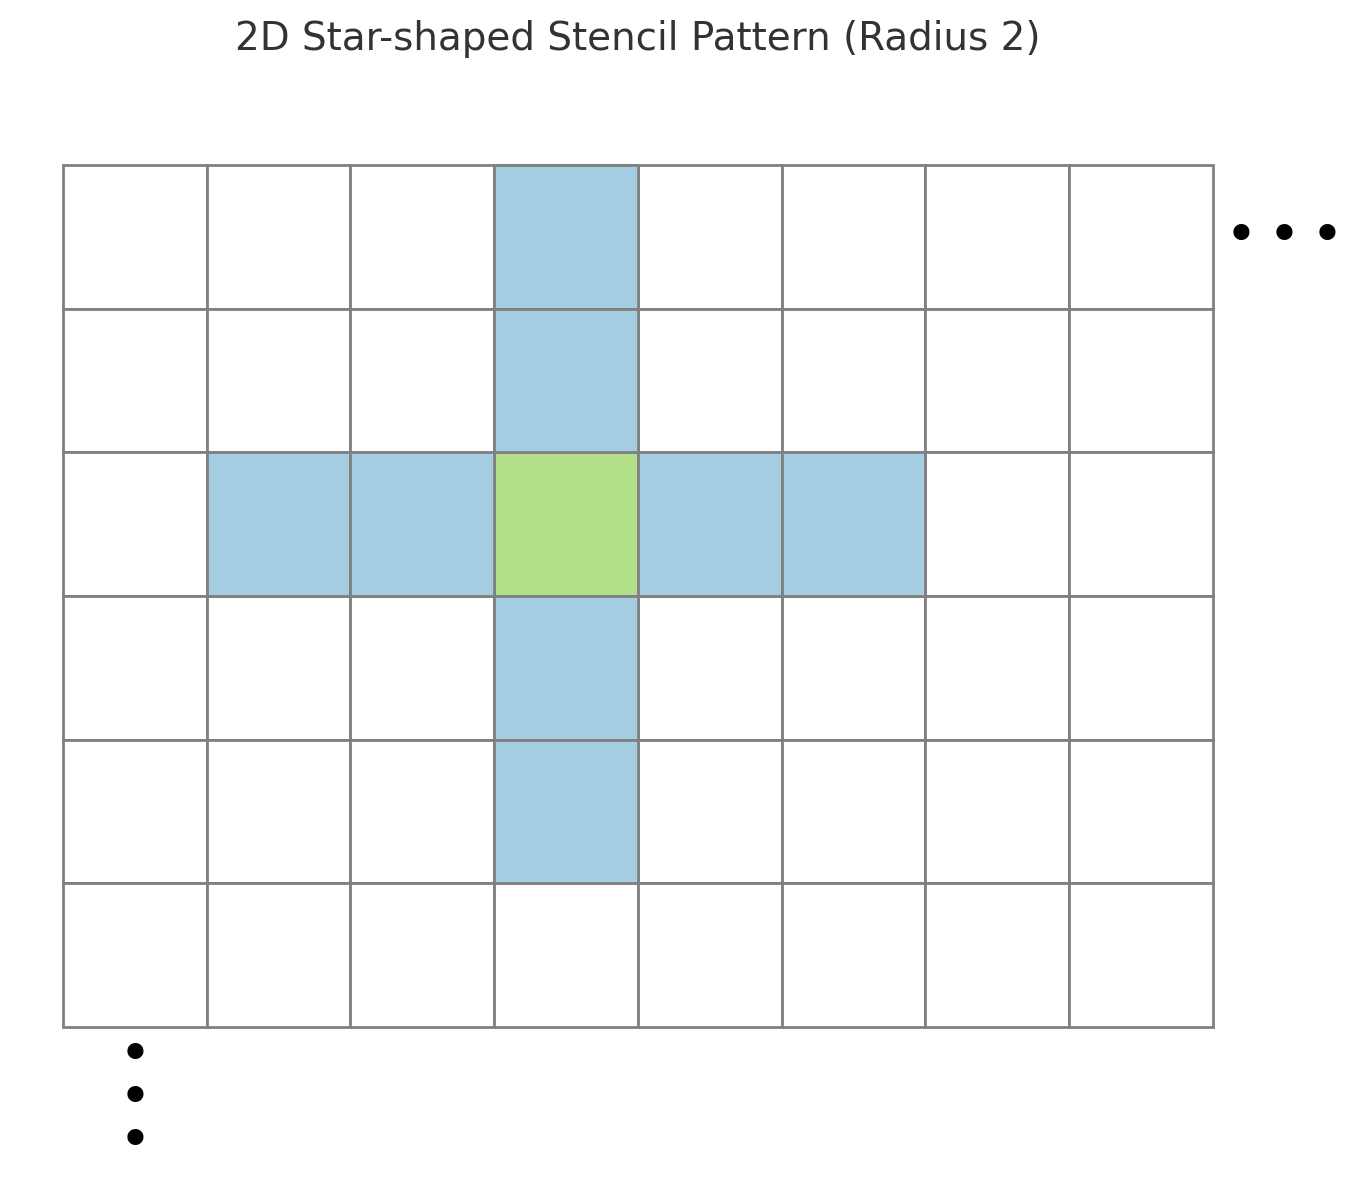
\includegraphics[width=0.5\linewidth]{stencil_visualization.png}
    \caption{A 2D star-shaped stencil pattern with radius 2}
    \label{fig:stencil_visualization}
\end{figure}

\section{The Cerebras Wafer-Scale Engine (\ac{wse})}
The Cerebras \ac{wse} has very distinctive characteristics compared to both \acp{cpu} and \acp{gpu}.
Instead of memory that is separate from the compute cores, the Cerebras \ac{wse} features several hundred thousand \acp{pe} that each consist of \qty{48}{\kilo\byte} of memory, a router for communication and a \ac{ce}. In contrast to traditional hardware, the memory consists solely of ultra-fast \ac{sram} with a bandwidth that supports two \qty{64}{\bit} reads and one \qty{64}{\bit} write per cycle. It is laid out into eight banks with specific restrictions on which banks can be accessed at the same time.

Each fabric router has a bidirectional link to the routers of the four neighboring \acp{pe} as well as to its corresponding \ac{ce}. All of these links have a bidirectional bandwidth of \qty{32}{\bit} per cycle. So-called colors define separate virtual communication channels and can be used to configure the data flow within the \ac{wse}. Specifically, one of 24 colors can be chosen for data leaving the \ac{ce} and for each router and color a set of directions to forward incoming data to can be specified. For the \ac{wse}-2, \numproduct{66 x 154} \acp{pe} form a die and \numproduct{12 x 7} dies reside on one \qty{300}{\mm} wafer, forming the \ac{wse}-2 with a staggering \num{853104} physical \acp{pe}. Distinct from traditional production processes, the dies are not cut, but kept together on the wafer and are linked so that the communication between \acp{pe} not only works within each die but also between dies.
The data flow between \acp{pe} can be defined through 24 static routes called colors \cite{lie2023cerebras}.
Due to imperfect yield, some \acp{pe} are non-functional.
Cerebras solves this problem by routing around these \acp{pe}. 
To make this work, the hardware includes about 1\% spare \acp{pe} so that the number of enabled \acp{pe} is a bit lower. Furthermore, the \ac{wse}-2 contains \acp{pe} that are not available to the user, but are reserved for memory movement and other system functions \cite{tramm2024efficient}.
The Cerebras documentation suggests that the usable number of \acp{pe} might even change slightly from system to system \cite{cerebras_gemv_tutorial}. \citeauthor{tramm2024efficient} \cite{tramm2024efficient} find the user-programmable number of \acp{pe} for the \ac{wse}-2 to be \numproduct{750 x 994}, which is the number we use throughout our work. For the \ac{wse}-3, the official documentation states the fabric dimensions to be \numproduct{762 x 1176}, and while this does not include the spare cores, it is not clear whether the number of user-programmable \acp{pe} is the same or might be slightly lower. In the absence of official numbers, we use these throughout our work. On the \ac{wse}, each \ac{pe} has its own clock, and while these all operate at the same frequency, they are not synchronized. Although the cores are designed to run at a frequency of \qty{1.1}{\giga\hertz} \cite{lie2023cerebras}, typical deployments run at a lower frequency of \qty{850}{\mega\hertz} for the \ac{wse}-2 \cite{tramm2024efficient} and \qty{875}{\mega\hertz} for the \ac{wse}-3. Therefore, we use these lower numbers for performance analysis throughout this work.

\begin{figure}[h]
    \centering
    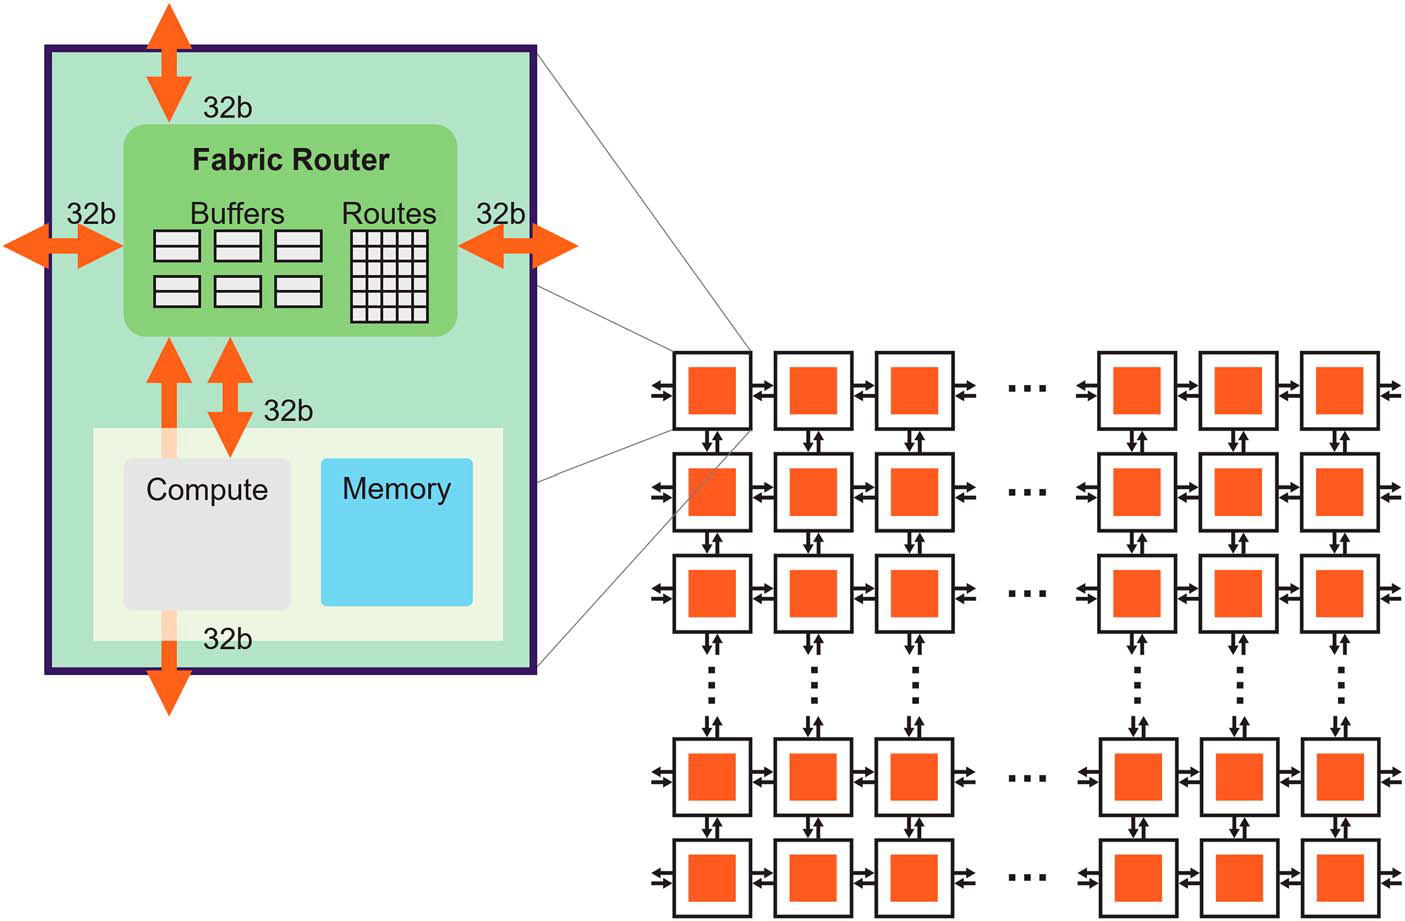
\includegraphics[width=0.5\linewidth]{wse2_pes_router.png}
    \caption{Schematic of \ac{wse}-2 processing elements arranged in a grid with interconnected routers \cite{lie2023cerebras}}
    \label{fig:wse2_pes_router}
\end{figure}

Each \ac{pe} allows the execution of certain instructions in parallel with \acp{simd} units. The maximum number of parallel instructions varies between instruction types and \ac{wse} generations. Table \ref{tab:simd_operations} shows the maximum \acp{simd} width for selected instruction types. As the \ac{wse} was originally designed for \ac{ai} workloads, the \acp{simd} units are optimized for half-precision floating-point operations, which are not suitable for \ac{hpc} workloads. 

\begin{table}[h]
    \centering
    \caption{Maximum \ac{simd} width for selected instruction types}
    \label{tab:simd_operations}
    \begin{tabular}{@{}llll@{}}
        \toprule
        Op code & description & \ac{wse}-2 & \ac{wse}-3 \\
        \midrule
        \texttt{@fadds} & 32-bit floating-point add & 2 & 4 \\
        \texttt{@fmuls} & 32-bit floating-point multiply & 1 & 1 \\
        \texttt{@fmach} & 16-bit floating-point multiply-add & 4 & 8 \\
        \texttt{@fmachs} & 16-bit floating-point multiply with 32-bit addition & 2 & 4 \\
        \texttt{@fmacs} & 32-bit floating-point multiply-add & 1 & 1 \\
        \texttt{@fmovs} & 32-bit floating-point move & 2 & 4 \\
        \bottomrule
    \end{tabular}
\end{table}

Custom kernels for the \ac{wse} are written in \ac{csl}, a low-level language based on Zig, extended with hardware-specific features.
One of its core features is the ability to define \acp{dsd} which define data access patterns including a base memory address, an offset, a stride and a length. They can be used for up to four-dimensional tensors. Specifically, there are four \ac{dsd} types: \texttt{mem1d\_dsd}, \texttt{mem4d\_dsd}, \texttt{fabin\_dsd} and \texttt{fabout\_dsd}. While \texttt{fabin\_dsd} and \texttt{fabout\_dsd} are used for fabric communication and \texttt{mem1d\_dsd} are used for one-dimensional arrays, \texttt{mem4d\_dsd} are somewhat unintuitively used for tensors with two, three, or four dimensions. The \ac{wse}-2 has 44 \acp{dsr} per \ac{pe}, which are hardware registers used to hold \acp{dsd}. These can be used directly as operands for instructions. Loading \acp{dsd} into \acp{dsr} is done automatically by the compiler, but can also be done manually and enables the programmer to optimize the code. Communication between \acp{pe} is handled with special fabin- and fabout-\acp{dsd}, describing data that is sent to or received from a neighboring \ac{pe}.

The routers contain a limited number of input and output queues, small physical buffers for incoming and outgoing data.

\ac{csl} has limited support for concurrency which is enabled by the use of tasks that are activated by events like completion of an asynchronous communication or computation. Due to the single thread of execution, there is no true parallelism within a single \ac{pe}.
